\chapter{FPGA Implementations}
\label{sec:chapter_3}

The hardware is introduced with some details of the implementations. The main FPGA side project is done in Xilinx System Generator which is a high level alternative with standard scripting languages like VHDL and Verilog. An overview to select the radio board and the clock chain inside will be described.\\
Main blocks in transmitter and receiver is defined and the mechanism for packet detection is illustrated in details.

\section{System Design in System Generator}
\label{sec_anasim}

Simulink® from The MathWorks® is a powerful graphical modeling system which allows complex systems to be designed using a block diagram methodology. Xilinx System Generator for DSP is a blockset for Simulink® which allows the modeling of fixed point systems which can be transformed into VHDL and targeted at an FPGA. Automatic generation of the bitstream is supported with the synthesis and implementation tools run from within the Simulink® environment.\\

\begin{figure}[h!]
\centering
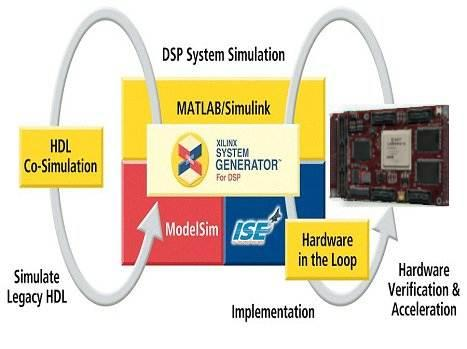
\includegraphics[width=10cm]{content/fig/systemGen.JPG}
\caption{System Generator Cycle.}
\label{fig:systemGen}
\end{figure}

Then main core of an an OFDM modulator and demodulator are the inverse FFT (IFFT) and FFT respectively. In 802.11a WLAN standard a 64-point transform with 52 of the subcarriers are carrying user data in a BPSK,
QPSK, 16-QAM or 64-QAM alphabet. The symbol rate in this systems is $20 MSym/s$. The OFDM symbol period
is $4 \mu s$, with $3.2 \mu s$ of this interval occupied by the 64-point FFT symbol and the additional $0.8 ps$ used for the cyclic prefix.\\

Figure \ref{fig:ofdm_system} shows the main scheme of an OFDM system in transmitter and receiver. Another block of Channel is a Additive White Gaussian Noise which is used in simulation only.\\
As you can see there are some others blocks which are necessary for system implementations. The whole system is connected to a main hard processor which is located in the FPGA. It is a ARM Cortex-A9 with maximum frequency of $666.66 MHz$. EDK processor represents the main processor which connected to the OFDM block by AXI protocol. 

\begin{figure}[h!]
\centering
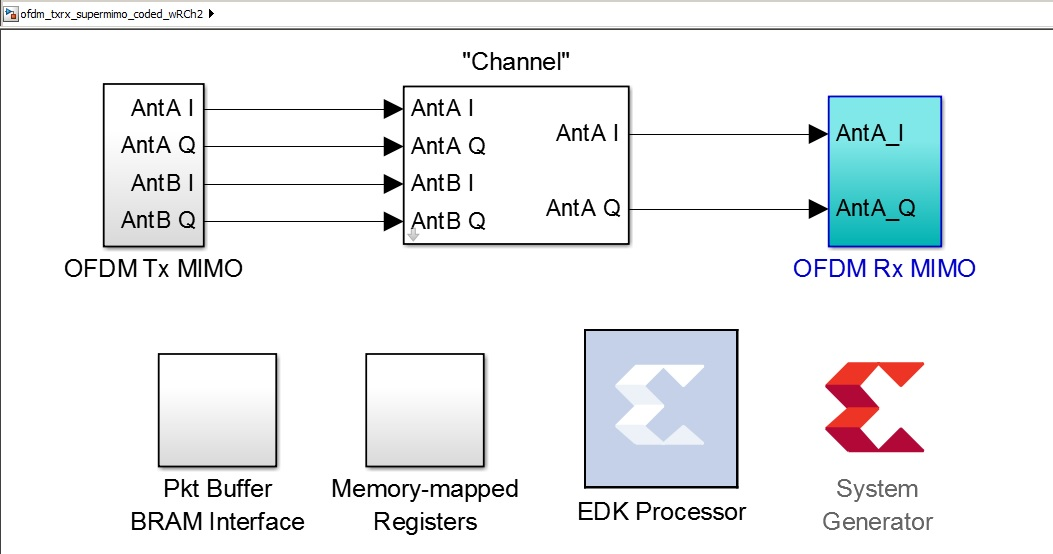
\includegraphics[width=10cm]{content/fig/system.JPG}
\caption{OFDM System..}
\label{fig:ofdm_system}
\end{figure}


Figure \ref{fig:tx_block} illustrates the transmitter which consists of many blocks. Controlling of the time we have \textit{TxControl} block for synchronization of the blocks. It also generate the semi-fixed preamble (LTS and STS) and the relevant Training signals for the system. \textit{Training Data} generates the training pattern which is used to estimate the channel frequency response.
The main clock is IFFT which convert the time-based signals into frequency. In the current picture we set a 64 point IFFT although the recent design it upgraded to 256 as a result of the strategy changes. The data captured by the IFFT blocks are integrated in the \textit{OutputBuffers}. \textit{OutputMuxes} block chooses between two possible antenna to transmit the stream. In \textit{PreSpin, Filters DACs}, some sub-blocks for soft gain and DAC preparation data are implemented. Besides, the are a generic block to rate change matter which can be activated by the processor.\\

\begin{figure}[h!]
\centering
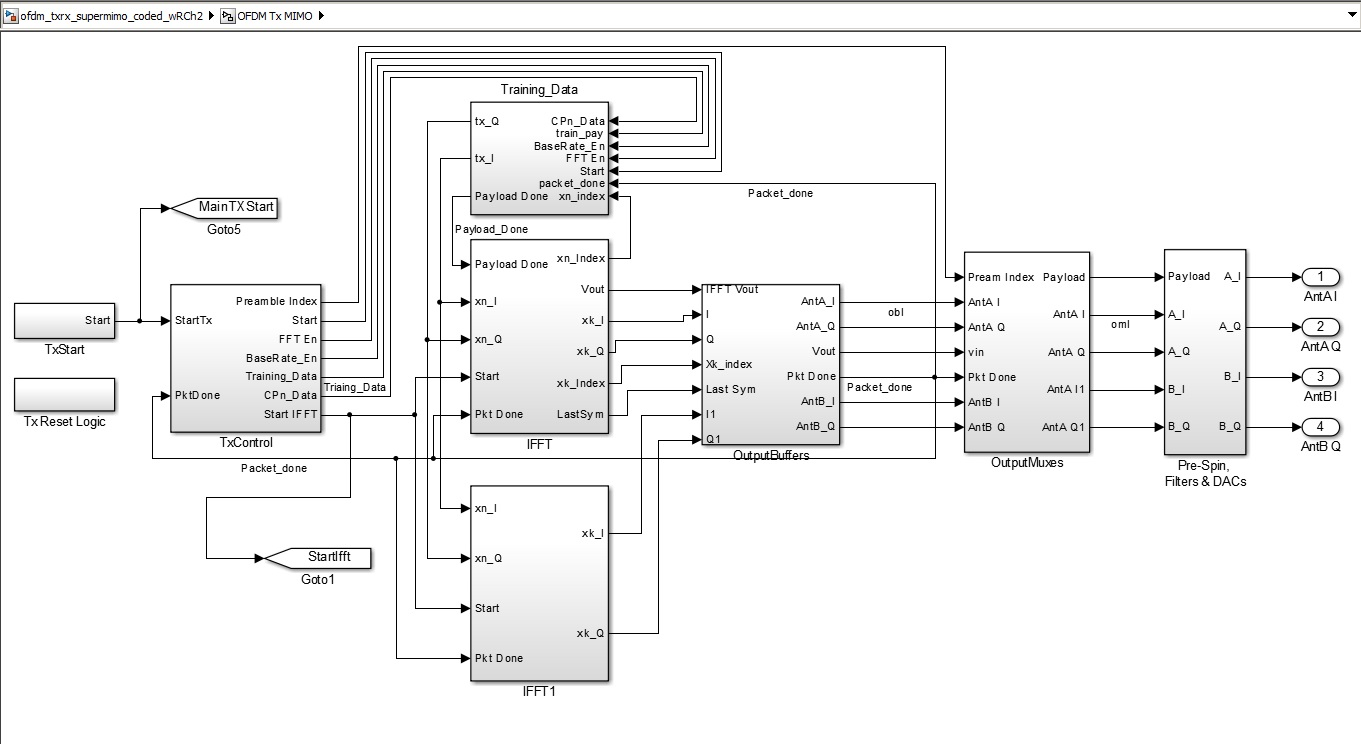
\includegraphics[width=\textwidth]{content/fig/txblock.JPG}
\caption{OFDM Transmitter Block.}
\label{fig:tx_block}
\end{figure}

Figure \ref{fig:rx_block} demonstrates the receiver block with its main blocks. The input signals enter into the device in a I/Q form from the analogue board. The is \textit{ADC inputs Antenna Selection} which we can switch between the two antennas and also the internal TX block which is reside in to the FPGA for the testing purposes. This block also adjust the input gain for the rest of the design. The frequency correction is done in the \textit{Coarse Freq Correction} using the STS stream.\\

\begin{figure}
\centering
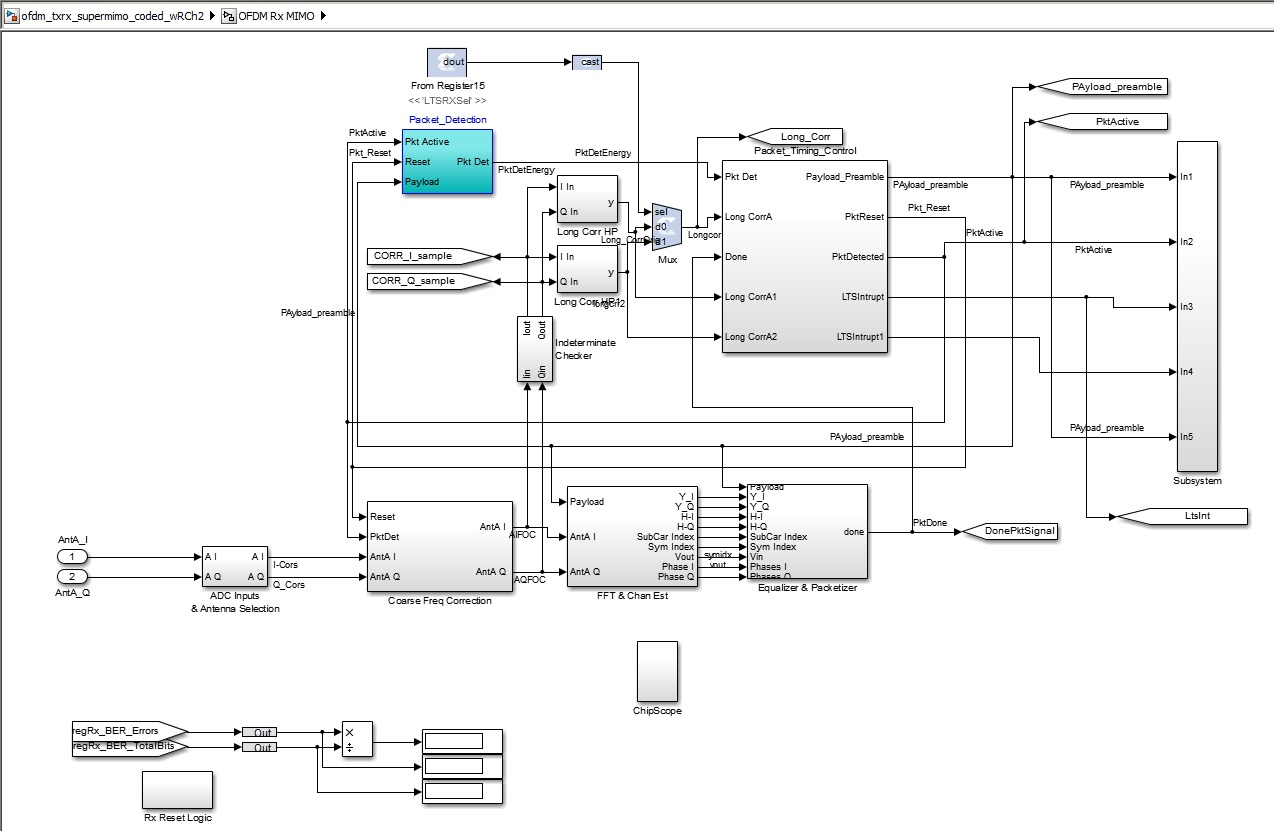
\includegraphics[width=\textwidth]{content/fig/rxblock.JPG}
\caption{OFDM Receiver Block.}
\label{fig:rx_block}
\end{figure}



In the \textit{Packet Detection} block an auto-correlation approach is done on the signal to detect the energy of the preamble in the beginning of STS shows in Figure \ref{fig:autocorrblock}. This is implemented based on the magnitude square of the both I/Q signals and comparing with a threshold after a sliding window. In other branch a multiplication of of the imaginary and real part with their 16 clock delayed version is calculated and the square magnitude in a sliding windows is detected. In \textit{Detection Decision} we use some other threshold to be ensure if the two cross correlation peaks are detected in the right time to signal the packet detection.

\begin{figure}
\centering
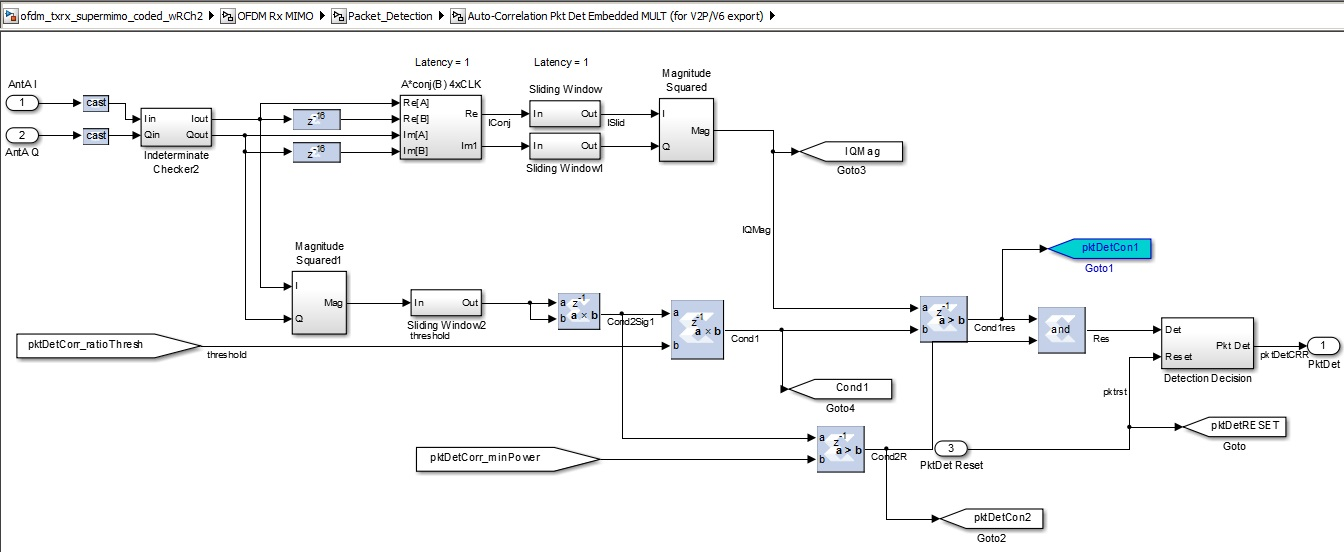
\includegraphics[width=\textwidth]{content/fig/autocorrblock.JPG}
\caption{Auto-Correlation Block.}
\label{fig:autocorrblock}
\end{figure}

\begin{figure}
\centering
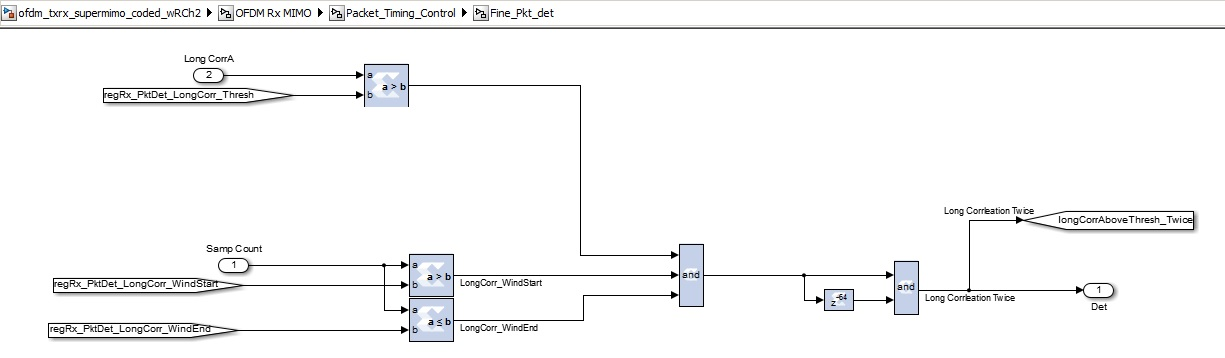
\includegraphics[width=\textwidth]{content/fig/fine_packetDetect.JPG}
\caption{Fine Packet Detection Block.}
\label{fig:fine_packetDetect}
\end{figure}

As described in Section \ref{section:channel_est}, the main part of the receiver is estimation of the channel which can be acquire by the LTS and training signal at the preamble. It is one of the most complex issue of the whole but the main part is shown in Figure \ref{fig:cmpx_div} and \ref{division}.\\

\begin{figure}
\centering
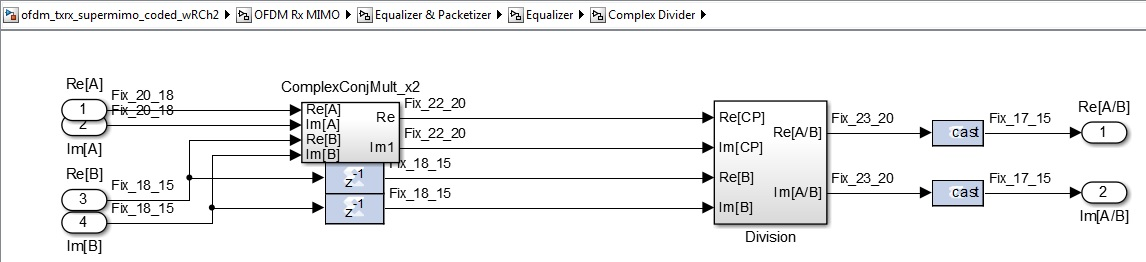
\includegraphics[width=\textwidth]{content/fig/cmpx_div.JPG}
\caption{Complex Division Block.}
\label{fig:cmpx_div}
\end{figure}

\begin{figure}
\centering
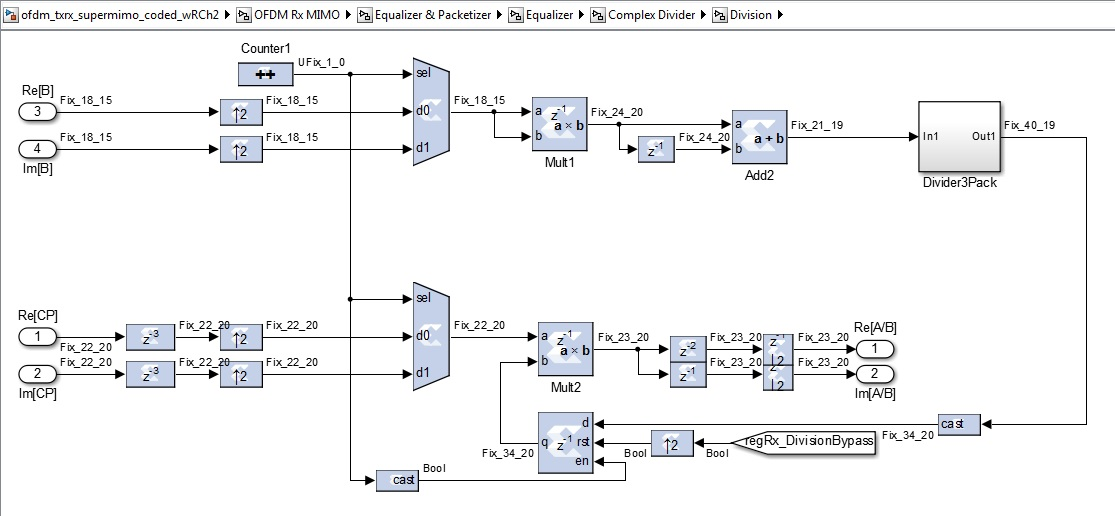
\includegraphics[width=\textwidth]{content/fig/division.JPG}
\caption{Division Block.}
\label{fig:division}
\end{figure}


\section{Hardware Introduction}
\subsection{FPGA Board}

The ZC706 evaluation board for the XC7Z045 All Programmable SoC (AP SoC) provides a hardware environment for developing and evaluating designs targeting the Zynq-7000 XC7Z045-2FFG900C AP SoC. The ZC706 evaluation board provides features common to
many embedded processing systems, including DDR3 SODIMM and component memory, a four-lane PCI Express interface, an Ethernet PHY, general purpose I/O, and two UART interfaces. Other features can be supported using VITA-57 FPGA mezzanine cards (FMC) attached to the low pin count (LPC) FMC and high pin count (HPC) FMC connectors. For details of architecture see Section \ref{fpga_arch}.\\

\begin{figure}
\centering
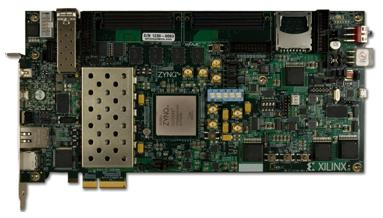
\includegraphics[width=12cm]{content/fig/ZC706.JPG}
\caption{ZC706 Evaluation Borad Block Diagram.}
\end{figure}

\begin{figure}
\centering
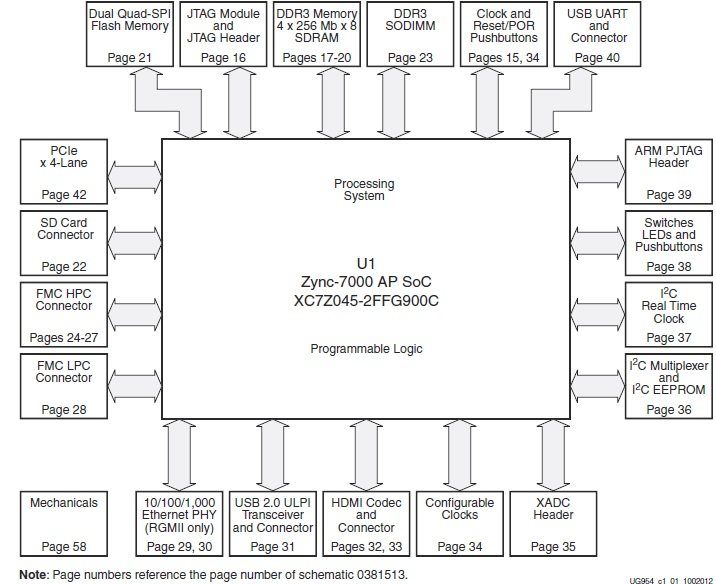
\includegraphics[width=12cm]{content/fig/zc706_block_diagram.JPG}
\caption{Xilinx Zynq-7000 SoC ZC706 Evaluation Kit}
\label{fig:zc706}
\end{figure}

\subsection{Radio Board}

The AD-FMCOMMS1-EBZ \cite{fmcomms1} high-speed analog module is designed to showcase one of the latest generation high-speed data converters. The AD-FMCOMMS1-EBZ provides the analog front-end for a wide range of compute-intensive FPGA-based radio applications.\\
The AD-FMCOMMS1-EBZ enables RF applications from 400MHz to 4 GHz. The module is customizable to a wide range of frequencies by software without any hardware changes, providing options for GPS or IEEE 1588 Synchronization, and MIMO configurations. When combined with the Xilinx ZC706, AD-FMCOMMS1-EBZ enables a variety of wireless communications functions at the physical layer, from baseband to RF. With up to 4 GB of flash storage space, 512 MB of RAM, Gigabit Ethernet interface (depending on the base platform). The platform offers enough flexibility for many applications, and supports streaming data, and standard web interfaces to analyze transmitted RF data.\\

\begin{figure}
\centering
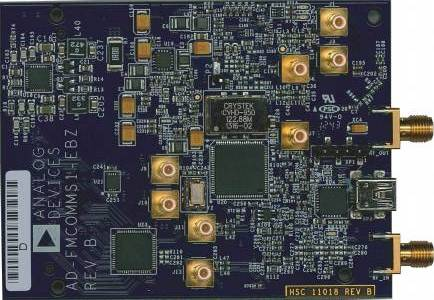
\includegraphics[width=10cm]{content/fig/fmcomms1.jpg}
\caption{AD-FMCOMMS1-EBZ (Radio Board)}
\end{figure}

\begin{figure}
\centering
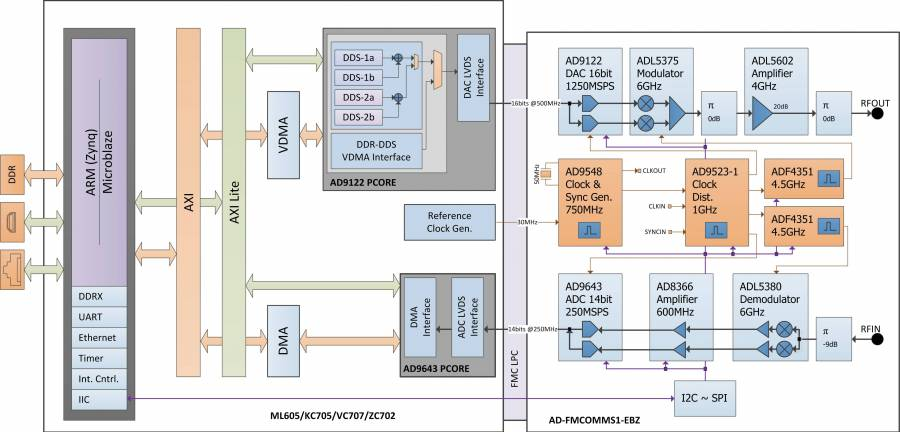
\includegraphics[width=15cm]{content/fig/fmcomms1Blockdiagram.jpg}
\caption{AD-FMCOMMS1-EBZ Block Diagram}
\label{fig:fmcomms1}
\end{figure}

\subsection{Clock Chain on FMCOMMS1}
Now, we discuss more about the clock chain and distribution mechanism on the board to find some meaningful number. As you can see in the figure, we configure the board and internal FPGA architecture to generate a 30MHz clock to the RF board. This 30MHz is just chosen because a relevant crystal mounted on the Zynq board and the all generated clock is supposed to be in-phased with it. This 30MHz is an input for AD9548 as a clock generator/synchronizer \cite{ad9548} which has a very precise PLL inside to generate a 20MHz.\\
The AD9548 generates an output clock synchronized to one of up to four differential or eight single-ended external input references. The digital PLL allows for reduction of input time jitter or phase noise associated with the external references. The AD9548 continuously generates a clean (low jitter), valid output clock even when all references have failed by means of a digitally controlled loop and holdover circuitry. AD9548 is a very complicated device to generate 20MHz with maximum precision.\\

\begin{figure}
\centering
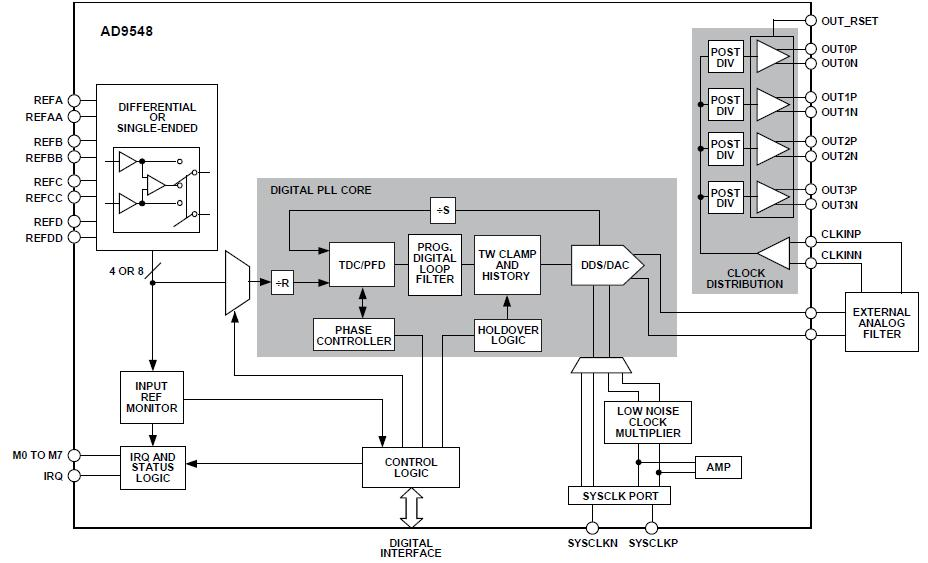
\includegraphics[width=15cm]{content/fig/ad9548BlockDiagram.JPG}
\caption{AD9548 Block Diagram}
\label{fig:ad9548}
\end{figure}

The next IC in the clock chain is AD9523-1 which is Low Jitter Clock Generator \cite{ad9523}. The AD9523-1 provides a low power, multi-output, clock distribution function with low jitter performance, along with an on-chip PLL and VCO with two VCO dividers. The on-chip VCO tunes from 2.94 GHz to 3.1 GHz. The AD9523-1 is defined to support the clock requirements for
long term evolution (LTE) and multicarrier GSM base station designs. It relies on an external VCXO to provide the reference
jitter cleanup to achieve the restrictive low phase noise requirements necessary for acceptable data converter SNR performance.\\
The input receivers, oscillator, and zero delay receiver provide both single-ended and differential operation. When connected to a recovered system reference clock and a VCXO, the device generates 14 low noise outputs with a range of 1 MHz to 1 GHz, and one dedicated buffered output from the input PLL (PLL1). The frequency and phase of one clock output relative to another clock output can be varied by means of a divider phase select function that serves as a jitter-free, coarse timing adjustment in increments that are equal to half the period of the signal coming out of the VCO.\\
In  our chain we have a 80MHz VCXO connected to AD9523-1. It is supposed to generated 40MHz for ADC, DAC and also the main OFDM architecture FPGA program. You can see the specification of the crystal oscillator in Figure \ref{fig:cvhd} \cite{cvhd} .\\

\begin{figure}
\centering
\includegraphics[width=10cm]{content/fig/cvhd.JPG}
\caption{CVHD-950 Ultra Low Phase Noise Oscillator}
\label{fig:cvhd}
\end{figure}


\section{Expectations for CFO on FMCOMM1}

In implementation of an OFDM chain, we should have good understanding the range of carrier frequency offsets which can be expected on our hardware platform. Our RF board foundation is based on FMCOMMS1. As a result, the elements in term of phase -noise and CFO should be studied. The main RF frequency refrence is a Crystek CVHD-950 (VCXO). This VCXO provides a clock signal at a nominal frequency of 80 MHz. Actual output frequency varies as a function of multiple factors, and is only specified by the manufacturer with some tolerance. The CVHD-950 is specified with a frequency tolerance of $\pm$4 ppm. Thus, we must design for a reference frequency of 80$\pm$0.000320 MHz. Imagine our target RF carrier frequency is 2452 MHz which implies 2400 MHz$\pm$4 ppm (or 2400$\pm$0.009600 MHz).\\
The worst case CFO will occur when the transmit and receive nodes operate at opposite ends of this range. Thus, for operation in the 2.4 GHz band our OFDM transceiver design must be ready to handle any carrier frequency offset up to $\approx$20 kHz.


\section{Time Domain CFO Correction}
Prevention of the degradation of CFO, the receiver should estimate and correct the offset in the time domain before the FFT block. The FFT block translates the received signal into the frequency. Regarding to the variety issue of OFDM, many estimation algorithms have been proposed.\\

\section{Carrier Frequency Offsets}
\label{sec_simstruct}
As a result of the frequency variation between local oscillators of the transmitter and the receiver nodes that generate the carrier signals, carrier frequency offsets (CFO) is happened. It causes when the baseband signal is going to be translated to RF. The issue is understood well but the impact to overcome CFO and suppression this phenomena is always depend on the specific parameters of the given transceiver and the hardware.\\
The origin of the CFO effect is studied in this section. We explore in a specific scenario of OFDM and the impact on the hardware design. Both simulation and experiments will be demonstrated and the CFO estimation and compensation is described.\\

\section{FPGA Architecture}
\label{fpga_arch}
Based on the Xilinx All programmable SoC architecture, the Zynq-7000 All Programmable SoCs \cite{zynq} enable extensive system level differentiation, integration, and flexibility through hardware, software, and I/O programmability. Using the Zynq-7000 platform, you can design smarter systems with tightly coupled software based control and analytic with real time hardware-based processing and optimized system interfaces.\\
As you can see in Figure \ref{fig:zynq_inside} the foundation of Zynq-7000 is divided into two main parts. Firstly, Processor System which are two ARM processors and the fixed implemented peripherals. The rest are just the raw Programmable Logic which the main OFDM physical layer is implemented inside. We should build the gates, DSP and RAM in this region by VHDL programming or System Generator software in Matlab environment.\\

\begin{figure}
\centering
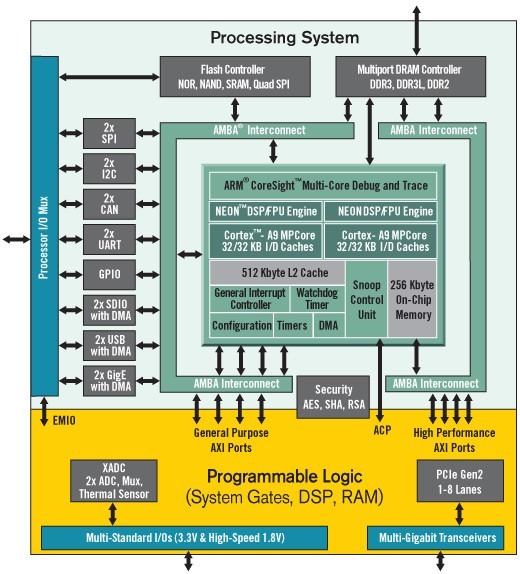
\includegraphics[width=12cm]{content/fig/zynq_inside.JPG}
\caption{Zynq-7000 Diagram}
\label{fig:zynq_inside}
\end{figure}

The block diagram of the design is illustrated in Figure \ref{fig:design_block_diagram}. We activate one of the ARM processors. In the TX chain, a PC sends a packet data via the Ethernet port to Zynq-7000. The EMAC block receives the packet and DMA it into the RX Block RAM which is divided into $32$ bank with size of $2K \times 64-bit$ which realize a Circular Buffer to relief the burst data stream enters from the asynchronous Ethernet port. As the OFDM block works in $40 MHz$ and each $2K$ block reading takes maximum $50\mu s$ for the EMAC and OFDM-PHY pessimistically, the tolerance of the Ethernet stream will be $\dfrac{32 \times \ 64b}{50\mu s} = 40Mbps$ which proves good number of banks. The offset pointer of reading and writing by DMA MAC which is govern under a scatter-gather scheme and the OFDM-PHY is controlled by the ARM.\\

\begin{figure}
\centering
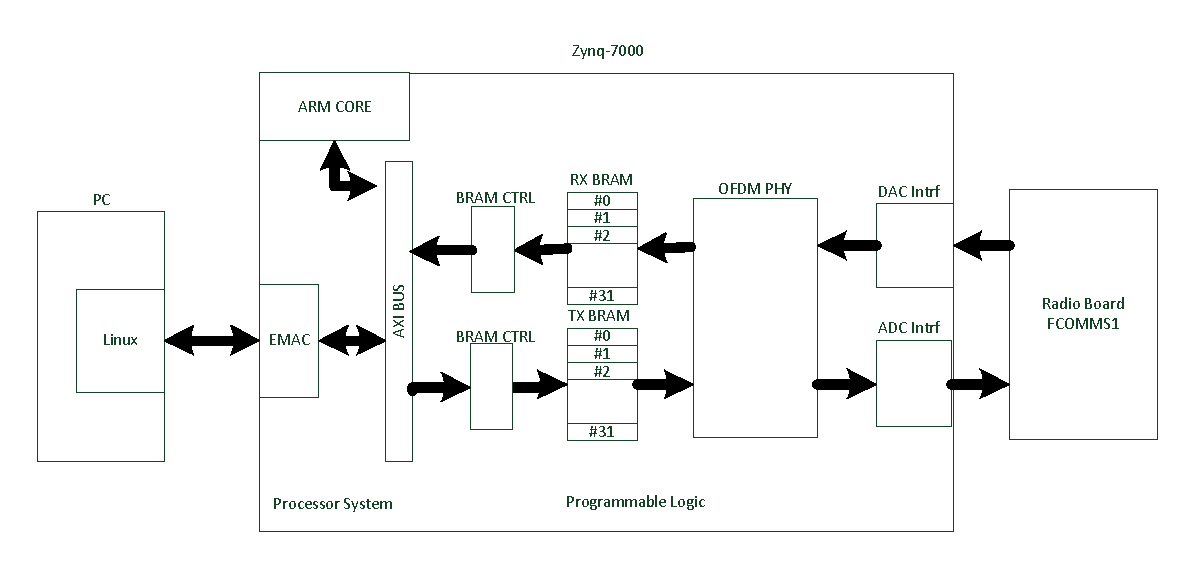
\includegraphics[width=\textwidth]{content/fig/sys_block_diagram.pdf}
\caption{Design Block Diagram}
\label{fig:design_block_diagram}
\end{figure}

As you can see in the block diagram the connection bridge between the Processor System and the Programmable Logic in the Zynq architecture can be AXI protocol. You can find the detail of AXI at ref..... There are some other communication protocols but in the Zynq design AXI works optimum.
For easier programming issues in PC side, we used Linux Virtual Machine inside a Windows OS. It is very helpful because this configuration prevents unnecessary data exchange of the system and helps us to have a real estimation of the bit rate.\\

\section{Test Methodology}
The configuration set-up is consisted of two Zynq board each carrying a FMCOMMS1 radio board. They are connected to two individual PC via Ethernet cables as shown in Figure \ref{fig:hardware_setup}.\\

\begin{figure}
\centering
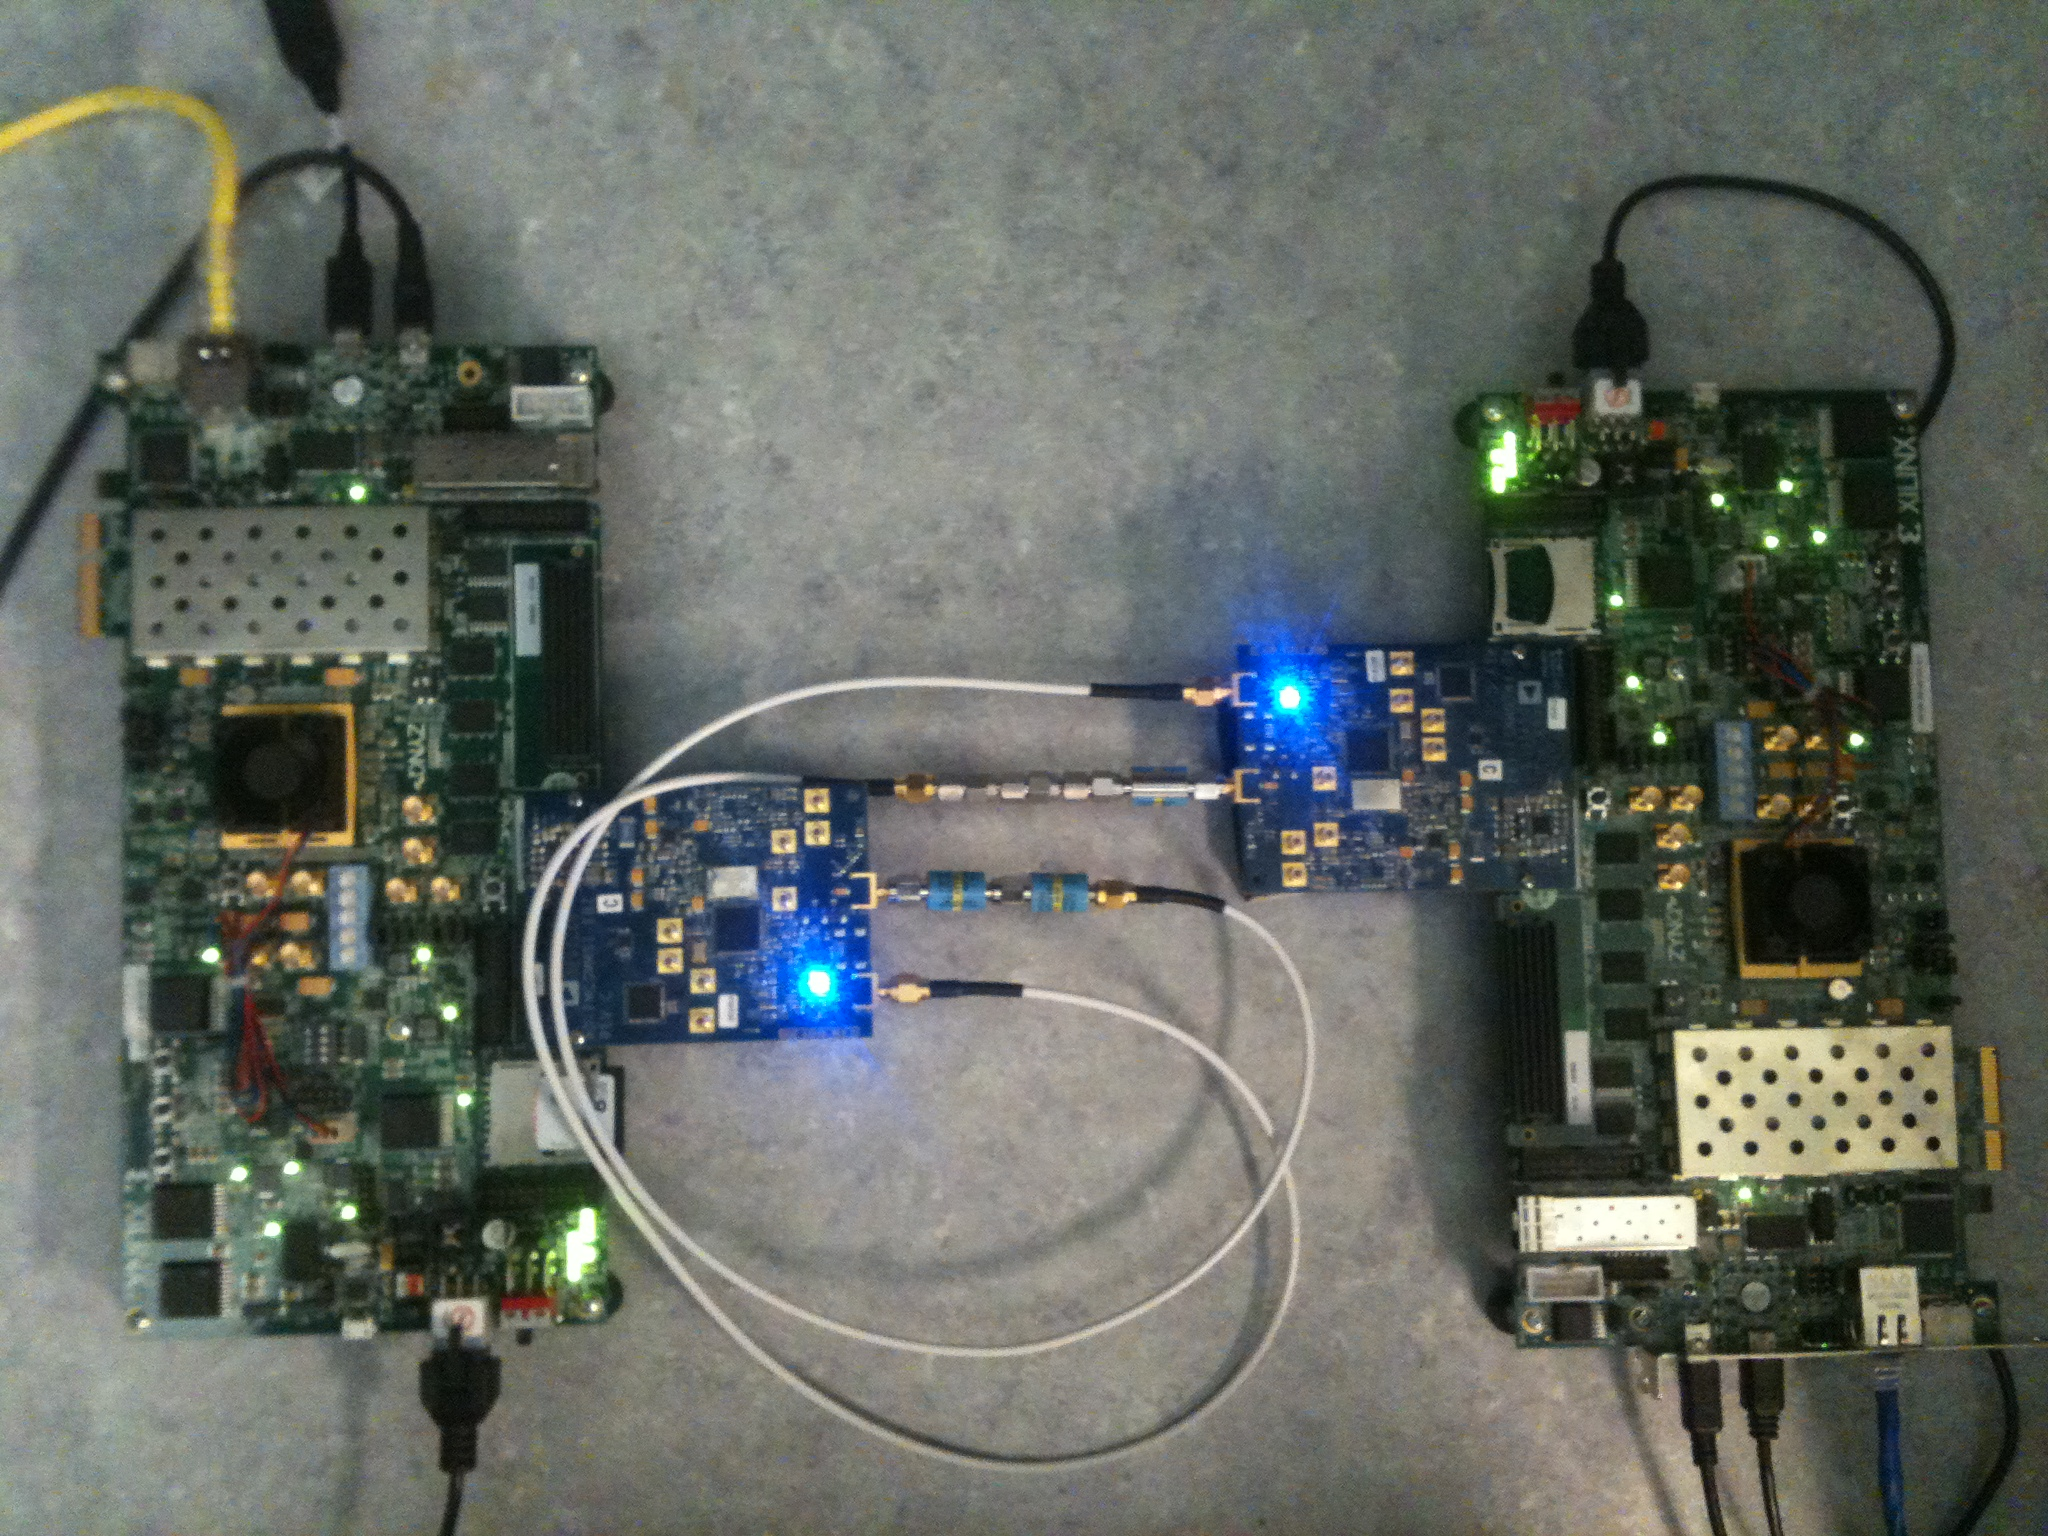
\includegraphics[width=\textwidth]{content/fig/hardware_setup.JPG}
\caption{Hardware set-up}
\label{fig:hardware_setup}
\end{figure}

This configuration should be tested partially and have realistic estimation of the maximum possible bit-rate and then calculate SNR of channel. Having engineering steps to examine each hardware block, we check the loops illustrated in Figure \ref{fig:design_block_diagram}.\\
The maximum bit rate we could reach to exchange via Ethernet peripheral of the Zynq board which is called EMAC is $600 Mbps$. This was a time consuming task to reach to this bit rate considering the complicated Direct Memory Access mechanism implemented in near contact of EMAC inside of ARM processor. Fortunately, there were many useful application examples dedicated by Xilinx but still it should study many document to understand the scheme in RX and TX of Ethernet.\\
Next, the correct configuration of the two TX and RX BRAMs are checked by directly data replacement between the two banks specified by the ARM processor. This was an important step because the maximum data rate is very depends on the correct data reading and writing into these two blocks. There is an useful functionality of the RAM which is designed also in Zynq-7000 that called Error-Correction Code (ECC). This is a type of computer data storage that can detect and correct the most common kinds of internal data corruption. ECC memory is used in most computers where data corruption cannot be tolerated under any circumstances, such as for scientific or financial computing. The two BRAMs communicate with AXI Bus via an BRAM controllers. The configuration of the BRAMs and the controllers should be set accordingly.\\
The main part of the project is dedicated of the OFDM-PHY block with its sophisticated details.\\
